\section*{Methods}
\setcounter{tocdepth}{2}
\tableofcontents
\section{Asteroseismic Methods}
\subsection{Asteroseismic Data}
For our asteroseismic power spectrum data we used the unweighted power spectra from the KASOC pipeline \cite{handberg+lund2014}\footnote{Obtainable from the \href{http://kasoc.phys.au.dk/}{KASOC} webpage.}. We did not apply any additional treatment to these data. For 16 Cyg A \& B (KIC 12069424 and KIC 12069449) we used the KEPSEISMIC lightcurves \cite{garcia+2011}\footnote{Obtainable from \href{https://archive.
		stsci.edu/prepds/kepseismic/}{MAST}.}, which have significantly better signal-to-noise for these two stars.

For our sample, we used the asteroseismic ages obtained by \texttt{BASTA} \cite[BAyesian STellar Algorithm]{silvaaguirre+2015} in the Kages and LEGACY catalogues. These ages have been obtained by comparisons of measured oscillation properties to stellar models, accounting for an expanded range of metallicities. \texttt{BASTA} is thoroughly compared to four other seismic modelling techniques in \cite{silvaaguirre+2017}. While uncertainties found through \texttt{BASTA} are typically higher than for other techniques, only \texttt{BASTA} and \texttt{ASTFIT} \cite[Aarhus STellar Evolution Code]{christensen-dalsgaard2008} recover the radius, mass and age of the Sun, when applied to solar data. Although the uncertainties on \texttt{ASTFIT} ages are overall lower, they are not reported in \cite{silvaaguirre+2015} for the Kages sample. In order to maintain an internally consistent stellar age sample, we used age results from \texttt{BASTA} for both the Kages and LEGACY samples.

For our stellar masses we used asteroseismic model masses obtained by \texttt{BASTA} reported in Kages and LEGACY, in order to maintain internal consistency with the age measurements. We note that age and mass posteriors from \texttt{BASTA} are correlated, but chose not to account for the unpublished correlations in this work.
As described in the catalogue papers, for Kages stars atmospheric properties (\teff and \feh) were measured through high-resolution spectroscopy reported in \cite{huber+2013a}. For LEGACY stars, atmospheric properties were similarly taken from \cite{buchhave+latham2015} for most stars in the catalogue, and complemented by other values from the literature for the remaining stars \cite[see Table 3]{silvaaguirre+2017}.

\begin{figure*}
	\centering
	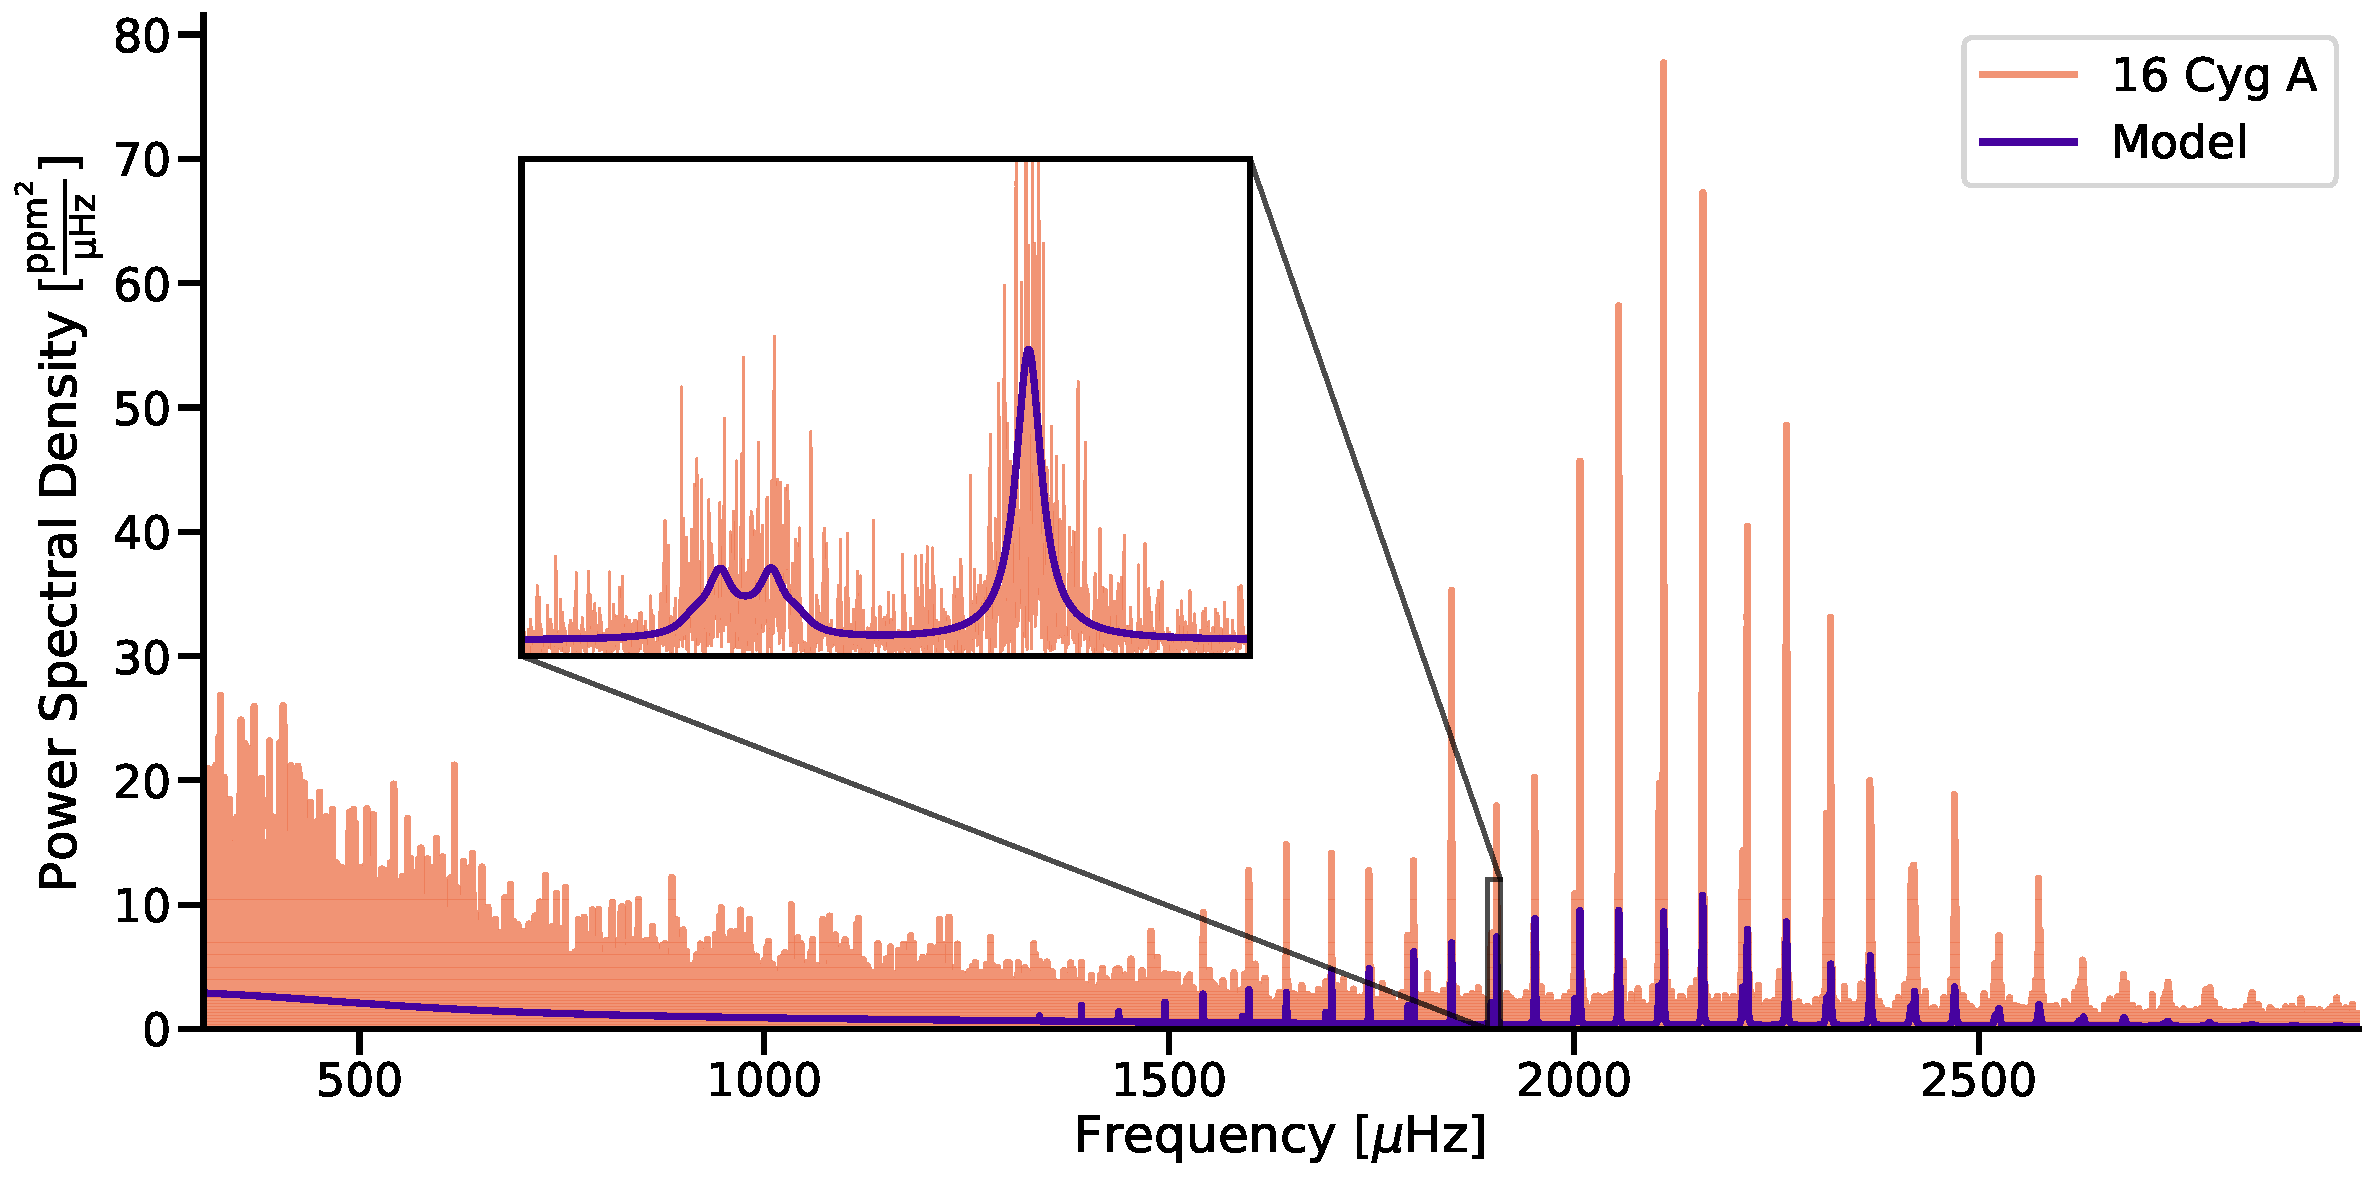
\includegraphics[width=.99\textwidth]{Images/modelfit.pdf}
	\caption{A power spectrum constructed from four years of \kepler observations of 16 Cyg A (KIC 12069424). Plotted over the top is the model resulting from the fit to the data described in this work. The model implements both the mode frequencies, seen on the right hand side of the plot, and the convective background, the effects of which are seen on the left. Low frequencies have been cropped out for clarity. \textit{Inset}: A zoom in on a radial (right) and quadrupole (left) ($\ell = 0, 2$) pair of modes. The quadrupole mode is split into five components by the star's rotation. Due to the star's inclination angle with respect to us, two out of five peaks are more distinct. The height and spacing of the mode components is a function of the star's rotational splitting ($0.56\, \mu\rm{Hz}$, equivalent to $P_{\rm rot} = 20.5\, \rm{days}$) and angle of inclination ($45^\circ$).}
	\label{fig:modelfit}
\end{figure*}


\section{Gyrochronology Methods}\label{s:gyro}
\subsection{Stellar Models}\label{ssec:models}
The braking models used in this work have several parameters that inform the rotational evolution. These are: a normalization factor to reproduce the solar rotation ($f_k$); a disk locking timescale ($T_{\rm disk}$) and period ($P_{\rm disk}$) which together regulate the stellar angular velocity during the pre-main sequence; the critical angular velocity that marks the transition from saturated (rapidly rotating) to unsaturated (slowly rotating) regimes ($\omega_{\rm crit}$), and the critical Rossby number, above which stars conserve angular momentum ($Ro_{\rm crit}$), mentioned above. $T_{\rm disk}$, $P_{\rm disk}$ and $\omega_{\rm crit}$ are calibrated to match the behavior in young open clusters, but have little impact on the rotational evolution beyond $\approx 1\, \rm{Gyr}$ in solar-mass stars. Both $f_k$ and $Ro_{\rm crit}$ affect the late-time evolution. Both models adopt $\omega_{\rm crit} = 3.4  \times 10^{-5}\, \rm{s}^{-1}$, $P_{\rm disk} = 8.1$, $T_{\rm disk} = 0.28$ and $f_k = 6.6$. In the weakened magnetic braking model, $Ro_{\rm crit} = 1.97$. For further details, see \cite{vansaders+pinsonneault2013} and \cite{vansaders+2016, vansaders+2019}.

Instead of comparing asteroseismic measurements of age and rotation directly to rotational models of individual stars, we instead compared them to synthetic populations based on rotational models, similar to those presented in \cite{vansaders+2019}, with some adaptations. To construct a synthetic population of rotating stars, \cite{vansaders+2019} applied the rotational braking laws described above to a galactic population model. Their approach used a TRILEGAL \cite{girardi+2012} Milky-Way simulation of the \kepler field, using the standard population values intended for this purpose from \cite{girardi+2015}. Stars from the TRILEGAL simulations were then drawn randomly in bins until they matched observations of stellar parameters of the \kepler field \cite{mathur+2017}. This aimed to replicate the \kepler selection effect, by ensuring the TRILEGAL population properties matched those observed in the \kepler field.

We used the same approach here, with two changes. First, we updated the distribution of stellar parameters matched to the TRILEGAL populations. Instead of \cite{mathur+2017}, we used the \cite{berger+2020} temperatures and luminosities, and 2MASS $K$-band magnitudes as our stellar parameter distributions for the \kepler field, which are more accurate following the use of \gaia DR2 parallaxes \cite{gaiacollaboration+2018}. The TRILEGAL simulation was matched to the \cite{berger+2020} sample using a nearest-neighbours approach (as opposed to binning), based on the density of stars on the HR diagram.

Second, we made further changes to account for possible binarity in the the \cite{berger+2020} sample. If the first step is performed blindly, blended binaries in the sample cause an overestimation of the number of old stars. In order to overcome this, we:

\begin{enumerate}
	\item blended the TRILEGAL stars with binary companions drawn from a flat mass-ratio distribution, using the binary fraction of \cite{raghavan+2010},
	\item recalculated the `observed' luminosities and magnitudes assuming that each binary pair was blended, and
	\item shifted these stars' temperatures following the $g$-$K$ relation presented in \cite{berger+2020}.
\end{enumerate}

This new distribution was used for the nearest-neighbour matching. Once drawn we dropped the binary companion and used the true TRILEGAL properties of those stars. For stars where the mass of the companion was $M < 0.4\, M_\odot$, binary contributions were ignored. Every binary was assumed to result in a blend, regardless of separation. This results in slightly more young stars than reality, because young, blended binary systems contaminate regions of the HR diagram where one expects to find old stars, and the number of blends is overestimated by assuming every binary system is a blend.

Our asteroseismic sample of stars with short cadence observations are subject to additional selection functions not included in the creation of the model populations above. We did \textit{not} explicitly account for these asteroseismic selection functions in our model, by design. Both the standard and WMB models contain stars with the same fundamental parameters (mass, radius, effective temperature, metallicity) but a different period based on the choice of rotational evolution prescription. Applying an asteroseismic selection function that depends on these fundamental parameters \cite{chaplin+2011} would apply an identical prior to both models, therefore providing no net effect on our posterior distribution. Additionally, we expected any seismic selection function to be relatively flat (and therefore uninformative) on a star-by-star scale, on which we run our model analysis (as opposed to a population scale, see below).

\subsection{Bayesian Mixture Models}
In order to determine whether weakened magnetic braking occurs on the main sequence, we compared our sample of seismic age and rotation, along with temperature, metallicity and mass, to the two stellar population models of the \kepler field adapted from \cite{vansaders+2019}, discussed above. Both stellar models were evaluated in a Bayesian framework, with the rationale of determining which of the two models (standard or WMB) is most likely to reproduce our observed data. Each model sample contained temperature (\teff), mass ($M$), age ($t$), metallicity ($\rm{[Fe/H]}$) and rotation ($P$) information.

In order to draw probabilistic inference about the models, we built a five-dimensional Kernel Density Estimate (KDE) of both model populations using the \texttt{statsmodels} package \cite{seabold+perktold2010}. We used a band-width (setting the resolution of the KDE) of $0.02\, M_\odot$ in mass, $10\, \rm K$ in \teff, $0.01\, \rm{dex}$ in $\ln(t)$, $0.01\, \rm{dex}$ in $\rm{[Fe/H]}$ and $0.01\, \rm{dex}$ in $\ln(P)$. Note that age and rotation were treated in log space, where the posterior estimates from asteroseismology more closely resemble normal distributions. This approach translates the population models to a probability distribution we can use in a Bayesian framework.

\begin{figure}
	\centering
	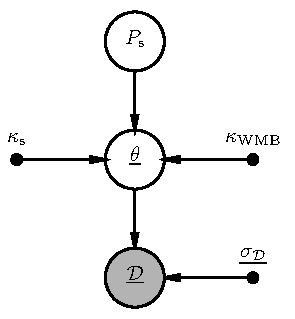
\includegraphics[width=0.45\textwidth]{pgm_models.pdf}
	\caption{A probabilistic graphical model (PGM) represented algebraically in Equation \ref{eq:modelll}. The shaded circle indicates observed data, and solid black points represent other fixed information, such as the KDEs and observational uncertainties. The remaining circles represent parameters. The underline indicates that the symbol represents a set of parameters or data. Here, $\kappa_{\rm{s}}$ and $\kappa_{\rm WMB}$ represent the KDEs of standard and WMB model populations respectively. $P_{\rm{s}}$ is the mixture model weighting factor. The latent parameters $\underline{\theta}$, our observations $\underline{\mathcal{D}}$ and their uncertainties $\underline{\sigma_{\mathcal{D}}}$ include temperature (\teff), mass ($M$), log-age ($\ln(t)$), metallicity (\feh) and log-rotation ($\ln(P)$). This model is \textit{hierarchical}, as all the latent parameters are drawn from the common probability distribution set by $P_{\rm{s}}$ and described in Equation \ref{eq:mixturell}.}
	\label{fig:pgm}
\end{figure}

We evaluated our data against both models simultaneously by treating the data as being drawn from a mixture of both model KDEs. In this mixture model structure, the two KDEs were modulated by a weighting factor, $P_{\rm s}$. In the limit $P_{\rm s} \rightarrow 1$, the data are most likely drawn from the standard model. In the limit $P_{\rm s} \rightarrow 0$, the data are most likely drawn from the WMB model.

The posterior probability of obtaining $P_{\rm s}$ and additional parameters $\theta$ given our data $\mathcal{D}$ is $p(P_{\rm{s}}, \theta | \mathcal{D})$. Using Bayes equation, we can express this as:

\begin{equation}\label{eq:modelll}
	p(P_{\rm{s}}, \theta | \mathcal{D}) \propto p(\mathcal{D} | \theta)\ p(\theta | P_{\rm{s}}, \kappa_{\rm{s}}, \kappa_{\rm{WMB}})\ p(P_{\rm{s}})\, ,
\end{equation}

\noindent where $\kappa_{\rm{s}}$ and $\kappa_{\rm{WMB}}$ are the KDE functions for the standard and WMB models respectively, and $\theta$ here are parameters, $\theta = \{M, \teff, \ln(t), \feh, \ln(P)\}$. As done above for the asteroseismic model, the parameters $\theta$ may be referred to as latent parameters, as they form a step between the parameter we want to infer ($P_{\rm{s}}$) and our data. Using this approach allowed our model to properly take into account the observational uncertainties on the data.

The second component on the right hand side of Equation \ref{eq:modelll} describes the probability of obtaining our latent parameters $\theta$ given our KDEs and the mixture model weighting parameter $P_{\rm s}$, and is described by the mixture model

\begin{equation}\label{eq:mixturell}
	p(\theta | P_{\rm{s}}, \kappa_{\rm{s}}, \kappa_{\rm{WMB}}) = P_{\rm s} \times \kappa_{\rm s}(\theta) + (1 - P_{\rm s}) \times \kappa_{\rm WMB}(\theta)\, ,
\end{equation}

\noindent where all parameters are as described above. This probability function describes a distribution that is a mixture of both KDEs. While the KDEs are constant, $P_{\rm s}$ is a free parameter, and so the shape of this distribution can vary. The latent parameters $\theta$ are drawn from this distribution, and therefore from some combination of the two stellar models.

The first component in Equation \ref{eq:modelll} describes the likelihood of obtaining the parameters $\theta$ given our data and their observational uncertainty. It takes the form

\begin{equation}
	p(\mathcal{D} | \theta) = \mathcal{N}(\mathcal{D} | \theta, \sigma_{\mathcal{D}})\, ,
\end{equation}

\noindent a normal distribution evaluating the latent parameters $\theta$ against the observations, with observational uncertainty $\sigma_{\mathcal{D}}$. This approach means that in each parameter space (such as age), the age drawn from the stellar model mixture is entered into the likelihood equation with our static observations. The value of this equation (and thus the likelihood) will increase if $\theta$ is closer to the observations, and the mixture model will be modulated in a manner that maximises this probability, inferring whether one stellar model is more likely to produce our data than the other.

The final term, $p(P_{\rm s})$, represents the prior on the mixture model weight, which is uniform between 0 and 1. A visual representation of our model is shown in Figure \ref{fig:pgm}.

Typically, this model would evaluate all stars in our sample against the stellar models simultaneously for a single posterior estimate of $P_{\rm s}$. At 95 stars, in 5 parameter spaces, this totals 476 free parameters to marginalise over. This is not an issue for Hamiltonian Monte Carlo \cite[HMC]{betancourt+girolami2013}, however the use of KDE functions, over which a probabilistic gradient can not be measured, reduces HMCs effectiveness. Alternative Markov Chain Monte Carlo techniques \cite[MCMC]{foreman-mackey+2013} can more efficiently sample the KDE functions, but can not treat the large number of hierarchical parameters. To overcome this, we fit our model to each star to obtain an independent individual posterior distribution for $P_{\rm s}$, and multiplied these post hoc to obtain a combined posterior. This comes with the benefit of easily allowing us to calculate the combined posterior for different stellar classifications (see Section \ref{s:class}), at the expense of the ability to marginalise for a single value of $P_{\rm s}$ directly. 

\subsubsection{Fitting procedure}
The parameter space of the stellar models was reduced before calculating the KDEs. These cuts were made in $M$, $\teff$, $\ln(t)$ and \feh, removing any stars in the models that fell more than $3 \times \sigma_{\mathcal{D}}$ outside the observations. Our observables $M$, $t$ and $P$ have asymmetric uncertainties from the Bayesian asteroseismic analysis. We used the larger of the reported uncertainties on each parameter as $\sigma_{\mathcal{D}}$ in each parameter space. 

KIC 6278762 was excluded from this stellar model analysis, because its age fell more than $3\sigma$ outside of the highest age in the stellar models\footnote{This is a metallicity issue, as the oldest stars have metallicities outside the range of the rotational model grids.}, and KICs 7106245 and 8760414 were excluded for the same reason due to low metallicities outside the functional range of the stellar models (-0.99 and -0.92 respectively).

We fit our model Equation \ref{eq:modelll} using \texttt{emcee} \cite{foreman-mackey+2013}, using 32 walkers for a total of 7500 samples per walker, of which the first 2500 were discarded as a burn-in.

After fitting, we took a normalised histogram of the posterior estimate of $P_{\rm s}$ for each star, using 100 bins. In this histogram, each bin approximated the value of the posterior function for $P_{\rm s}$. The array of 100 bins for all stars were multiplied, resulting in an approximation of the joint posterior probability function for $P_{\rm s}$ given all stars in the ensemble.



\section{Results}
bla bla short shpiel about which values were included and which weren't

\section{Verifying asteroseismic results}
\subsection{Priors on rotational parameters}
In our Bayesian analysis, we have placed weakly informative priors on our sampled rotational parameters, $\nu_{\rm s}\sin(i)$ and $\cos(i)$ (see Section \ref{s:seismo}). The prior is especially important for the angle of inclination, which is hardest to infer from the data. We are able to validate the robustness of our asteroseismic results by confirming that their posterior distributions are data-dominated, and not prior-dominated. We can do so by comparing the $68\%$ credible regions of the posterior estimates of $\nu_{\rm s}\sin(i)$ and $i$ against the $68\%$ credible regions of their priors.

A comparison between prior and posterior is shown for 94 stars in $\nu_{\rm s}\sin(i)$, $i$ and $P_{\rm rot}$ in Figure \ref{fig:priors}, arranged by age. In the Figure, results with means and error bars that closely resemble the prior distribution can be interpreted as prior-dominated (i.e. poorly informed by the data). The projected splitting, $\nu_{\rm s}\sin(i)$, is overall well constrained, with only one star appearing prior dominated. This is expected, as the projected splitting is what we observe on the star before decoupling inclination and rotation. The angle of inclination $i$, sampled as $\cos(i)$, more closely follows the prior distribution in most cases. Combining the two, the rotation period $P_{\rm rot}$ has no stars directly corresponding to the effective prior on period, and globally follows a trend with increasing age. The three outliers with fast rotation at late ages (KICs 6603624, 8760414 and 8938364) are discussed in more detail in Section \ref{ssec:litcomp}.

The rotation rates as presented in this work are a product of our Bayesian sampling of both projected splitting and angle of inclination. As seen in Figure \ref{fig:priors} there are instances where $i$ or $\nu_{\rm s}\sin(i)$ closely resemble the prior (and are therefore prior-dominated). There are no cases of this when looking at the resulting period measurements, as they will have been informed by at least one strongly data-driven parameter (judging from Figure \ref{fig:priors}, commonly $\nu_{\rm s}\sin(i)$). From this, we conclude that our ensemble of asteroseismic rotation is not strongly dominated by the priors imposed on projected splitting and inclination in our Bayesian analysis.

\subsection{Comparisons to previous studies}\label{ssec:litcomp}
In order to validate our results, we compared our rotational parameters to those obtained in the literature, as well as those resulting from the work presented in LEGACY and Kages, which were unreported and received through private communication by the authors of the catalogue papers.

Comparisons with LEGACY and Kages are shown in Figure \ref{fig:legacykages} for projected splitting, inclination angle, and rotation period. In all three cases we show the fractional difference between the values obtained in this work and those from LEGACY and Kages. On the right of Figure \ref{fig:legacykages}, we show the distribution of the fractional differences for the three parameters.
The projected splitting is in good agreement with both studies, however LEGACY finds slightly lower $\nu_{\rm s}\sin(i)$ for the faster rotators, deviating from our work by over $1\sigma$. Neither LEGACY nor Kages used a spatially isotropic prior for the inclination angle in their analyses, instead opting for a uniform prior. As posterior estimates of inclination angle are only loosely data-driven, the introduction of an isotropic prior should result in our analysis reporting globally higher inclination angles. This effect is seen in the comparisons of both inclination angles and rotation rates for the LEGACY stars, where we find overall lower rotation rates compared to LEGACY for stars at very similar $\nu_{\rm s}\sin(i)$.

A number of stars are excluded from Figure \ref{fig:legacykages} and compared individually as extreme outliers: KICs 5094751, 6196457, 8349582, 8494142, 8554498, 105114430 and 11133306 all have fast rotation rates ($<5\, \rm days$) in Kages, but are found to have a broader spread of rotation rates in this work. At similar values for $\nu_{\rm s}\sin(i)$, Kages found much lower inclination angles with highly asymmetrical uncertainties. Based on a comparison between the summary statistics of these stars, we conclude that the results found in this work have better marginalised over inclination angle, improving our measure of rotation.

Conversely, KICs 6603624, 8760414 and 8938364 have extremely slow rotation periods in LEGACY, but extremely \textit{fast} ($<3\, \rm {days}$) in this work. KICs 8760414 and 8938364 are excluded from the gyrochronology analysis below based on checks for $\hat{R}$ and the number of effective samples. Both stars have ages greater than $10\, \rm Gyr$, making their fast rotation rates highly unlikely under any model of rotational evolution. The posterior estimate of $P$ for KIC 6603624 is well-defined in our analysis, but with an age of $7.8\, \rm Gyr$, its measured rotation of $1.2\, \rm days$ is also highly unlikely under any model of rotational evolution. The LEGACY estimate of rotation is similarly extreme at $378\, \rm days$. These three stars have the lowest inclination angles in our sample ($< 10^\circ$), at which point the power in the split components of the seismic modes is so low that it becomes difficult to probe the measure of splitting\footnote{The split components for these stars will have a height roughly 3\% of the central mode. For comparison, for the next lowest inclined star at $17^\circ$, this rises to $10\%$.}. In cases such as these with lower signal-to-noise, spurious peaks may be interpreted as split components.\\

\begin{figure*}
	\centering
	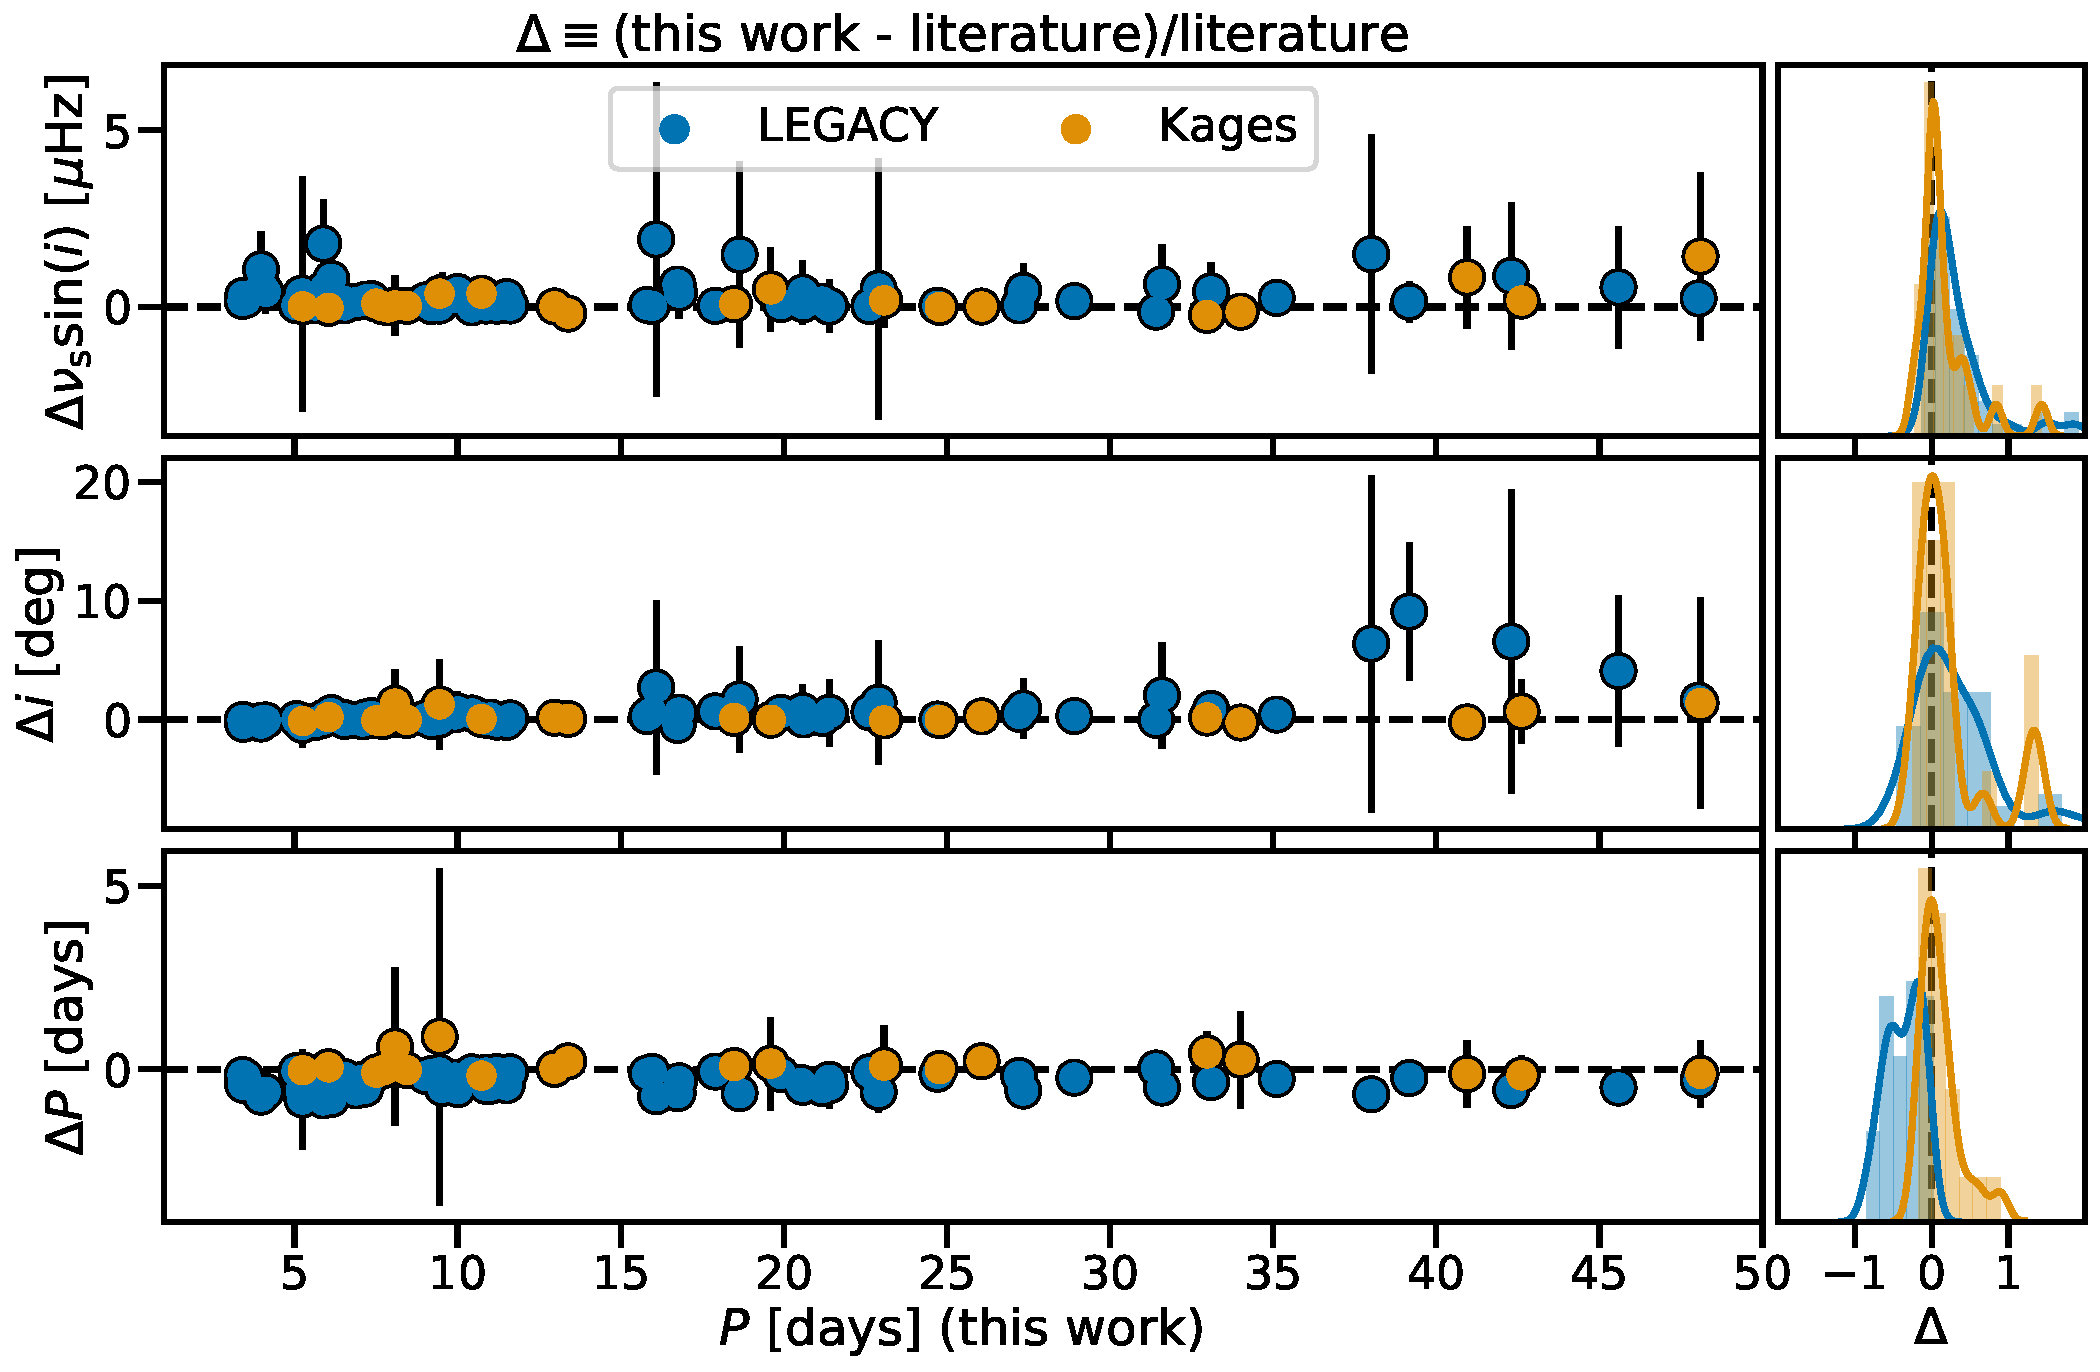
\includegraphics[width=\textwidth]{Images/litcomp_alt2.pdf}
	\caption{Comparisons between posterior estimates of rotational parameters from this work, LEGACY and Kages \cite[private communication]{davies+2016, lund+2017}. Fractional differences are plotted against stellar rotation obtained in this work. The $\Delta$ indicates the fractional difference betwen thsi work and the literature (i.e. stars above the zero-line have higher values in this work). The right hand panels the distribution of the fractional differences around the zero line. The colour legend is consistent throughout all panels. The x-axis units on the right hand panels are equivalent to the y-axis of the left hand panels. 10 stars have been omitted from this plot and are discussed in more detail in the text: KICs 5094751, 6196457, 8349582, 8494142, 8554498, 105114430 and 11133306 all have extremely low rotation periods in Kages, with high uncertainties. Conversely, KICs 6603624, 8760414 and 8938364 have extremely high rotation periods in LEGACY with low uncertainties. In cases where stars had asymmetric error bars, the larger of the two was used when propagating uncertainty for the purposes of this figure.}
	\label{fig:legacykages}
\end{figure*}

We also compared our asteroseismic estimates of stellar rotation with similar studies in the literature, shown in Figure \ref{fig:literaturecomp}. These included: \cite{davies+2015}, a study of the binary solar analogues 16 Cyg A \& B; \cite{nielsen+2015}, which our catalogue shares 5 stars with; and \cite{benomar+2018}, an asteroseismic study of differential rotation with which our catalogue shares 40 targets. For the latter, we used their reported splitting value $a_1$, which is equivalent to $\nu_{\rm s}$. 

Overall, Figure \ref{fig:literaturecomp} shows no strong disagreements between our asteroseismic measurements for stellar rotation and those from the literature. The scatter of the fractional differences lies cleanly around the zero line, with a mean and spread of $0.0_{-15.6}^{+16.4}\, \%$. The increase in uncertainty with period is due to more slowly rotating stars being more difficult to constrain using asteroseismology.
% The agreement within $1\sigma$ here is encouraging, indicating that these independent Bayesian analyses are finding appropriate uncertainties on these rotation measurements.

It is of note that 16 Cyg A, as reported by \cite{davies+2015} was found to be rotating slightly faster in our analysis (deviating within $2\sigma$), despite the fit being performed on the same data. We found an inclination angle that is slightly lower than \cite{davies+2015} for 16 Cyg A but a similar projected splitting, which would explain finding a lower value of rotation.

There are three outliers at low period in Figure \ref{fig:literaturecomp}: KICs 6603624, 8760414 and 8938364. These are the same targets found to be outliers in a comparison to the LEGACY and Kages measurements (see above), with anomalously fast rotation rates and low inclination angles. As these stars represent the lowest inclination angles in our sample, and were found to disagree with two independent studies, we opted to exclude them from the gyrochronology analysis, and to flag the rotation measurements for these three stars presented in this work.

\begin{figure}
	\centering
	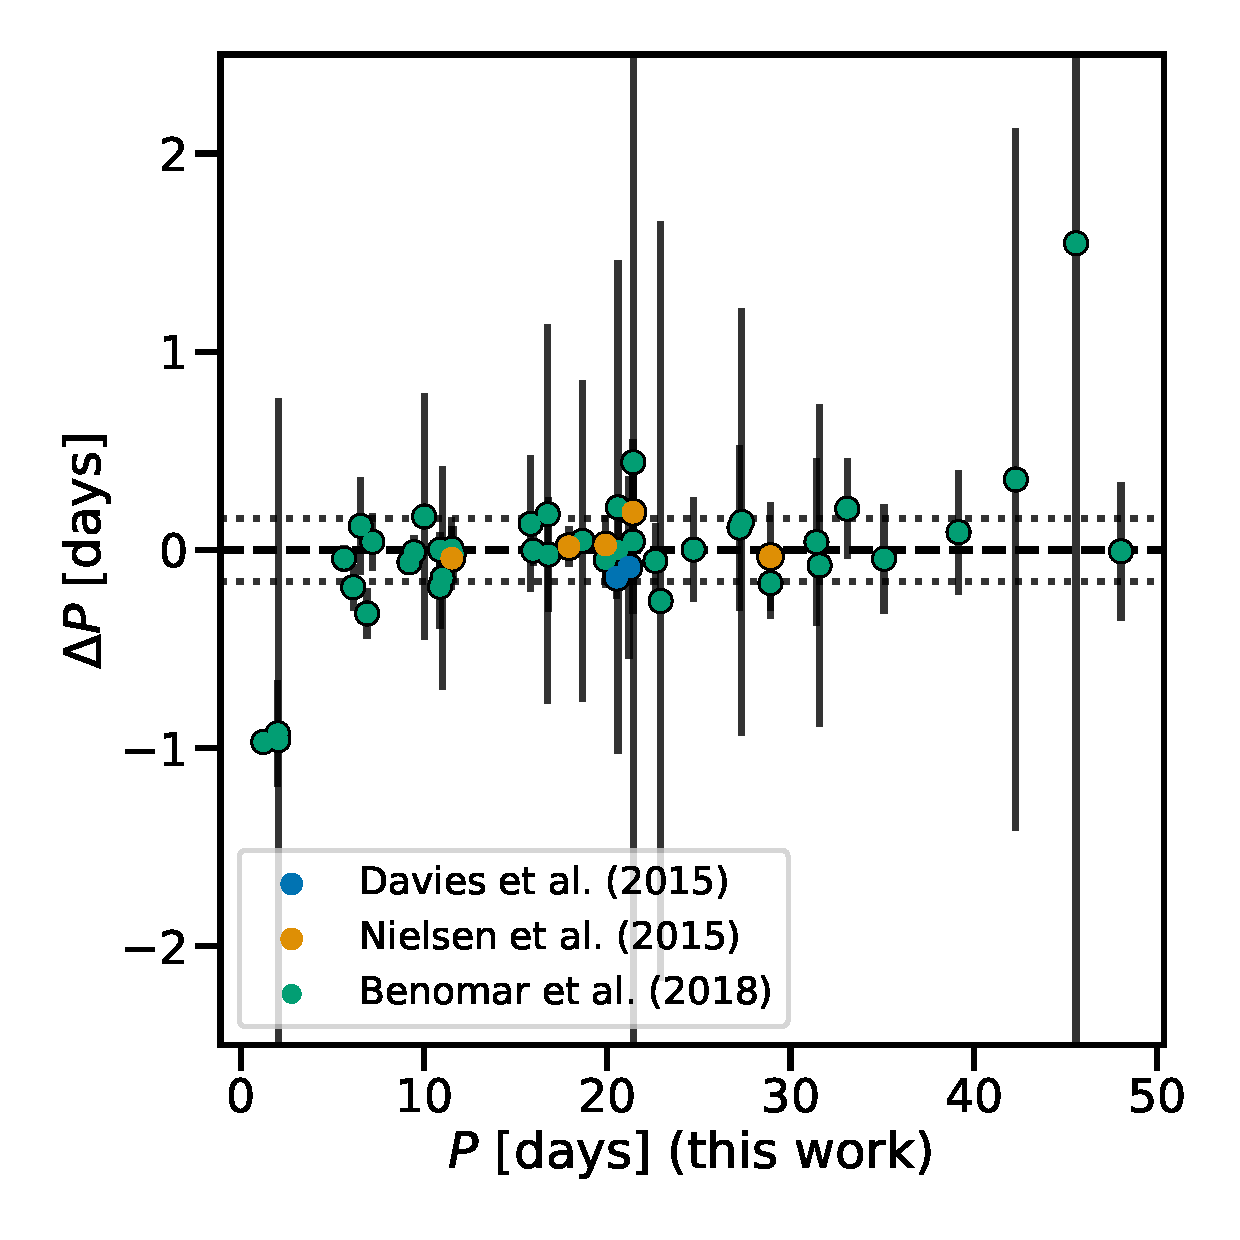
\includegraphics[width=0.49\textwidth]{Images/seis_comparison_rot_alt2.pdf}
	\caption{Fractional differences between posterior estimates of asteroseismic rotation period from this work. Literature sources are: \cite{davies+2015} (16 Cyg A \& B), \cite{nielsen+2015} (5 stars) and \cite{benomar+2018} (40 stars). We used the reported parameter $a_{1}$ from \cite{benomar+2018}, which represents the rotational splitting in the case of uniform latitudinal rotation in their model. The dashed line represents the median of the sample shown, with the dotted lines representing the $15.9^{\rm{th}}$ and $84.1^{\rm{st}}$ percentiles. In cases where stars had asymmetric error bars, the larger of the two was used when propagating uncertainty for the purposes of this figure.}
	\label{fig:literaturecomp}
\end{figure}

\subsection{Internal vs external rotation}
Different methods of rotation measurement probe different regions of stars. Asteroseismology of main sequence stars probes internal rotation in the near surface layers, where the observed p modes are most sensitive \cite{lund+2014}. Measurements of star-spot modulation instead probe the rotation rates of star spots on the surface. A distinct difference between rotation rates obtained through these different techniques would hold information about differential rotation (both latitudinal and radial) of near-surface layers, such as those we observe in the Sun \cite{beck2000}. 

\cite{nielsen+2015} performed a comparative analysis of 5 Sun-like stars observed with \kepler for which both star-spot modulation and asteroseismic rotation could be measured. They found no statistically significant difference between the two techniques.

Similarly, \cite{benomar+2015} performed an analysis on a larger sample of 22 stars. In this work they not only considered rotation rates from spots, but also spectroscopic measures of the projected surface rotation $\textrm{v}\sin(i)$, which they found to be more reliable. Comparisons with asteroseismic observations again showed no significant radial differential rotation.

With our expanded sample of asteroseismic rotation we can perform a similar analysis, to both validate our sample and probe radial differential rotation. Figure \ref{fig:vsinilit} shows a comparison between spectroscopic $\textrm{v}\sin(i)$ measurements as listed in LEGACY and Kages (left) and \cite{benomar+2015} (right). In these cases the asteroseismic $\textrm{v}\sin(i)$ has been calculated using our measure of asteroseismic $\nu_s\sin(i)$ and the known asteroseismic radii. Three stars (KICs 6603624, 8760414 and 8938364) have been excluded from this figure due to strong disagreements of measured rotation rates with the literature (see Section \ref{ssec:litcomp} above).

For the LEGACY and Kages sample, we find no strong deviation from the 1:1 line except at very low velocities, which is likely due to biases inherent to spectroscopic line broadening measurements \cite{doyle+2014, tayar+2015}. For the \cite{benomar+2015} sample stars lie a lot closer to the 1:1 line.
% , apart from one clear outlier. While we find no statistically significant difference between these observations, more in-depth studies of stars furthest away from the bisector in this sample may prove valuable in future work.

Overall, there appears to be a global offset where spectroscopic measurements of projected rotation appear faster than asteroseismic measures. Based on the LEGACY and Kages $v\sin(i)$ values, this offset is roughly $18\%$ (i.e. spectroscopic projected rotation rates are higher than asteroseismic rates). This offset is much smaller ($\sim5\%$) for the \cite{benomar+2015} sample, albeit for far fewer stars. These offsets are within the typical disagreement between spectroscopic methods, based on comparisons of projected rotation measurements for red giant stars \cite[see Figure 2]{tayar+2015}, especially at $< 5\, \rm{km\,s^{-1}}$.\\

\begin{figure*}
	\centering
	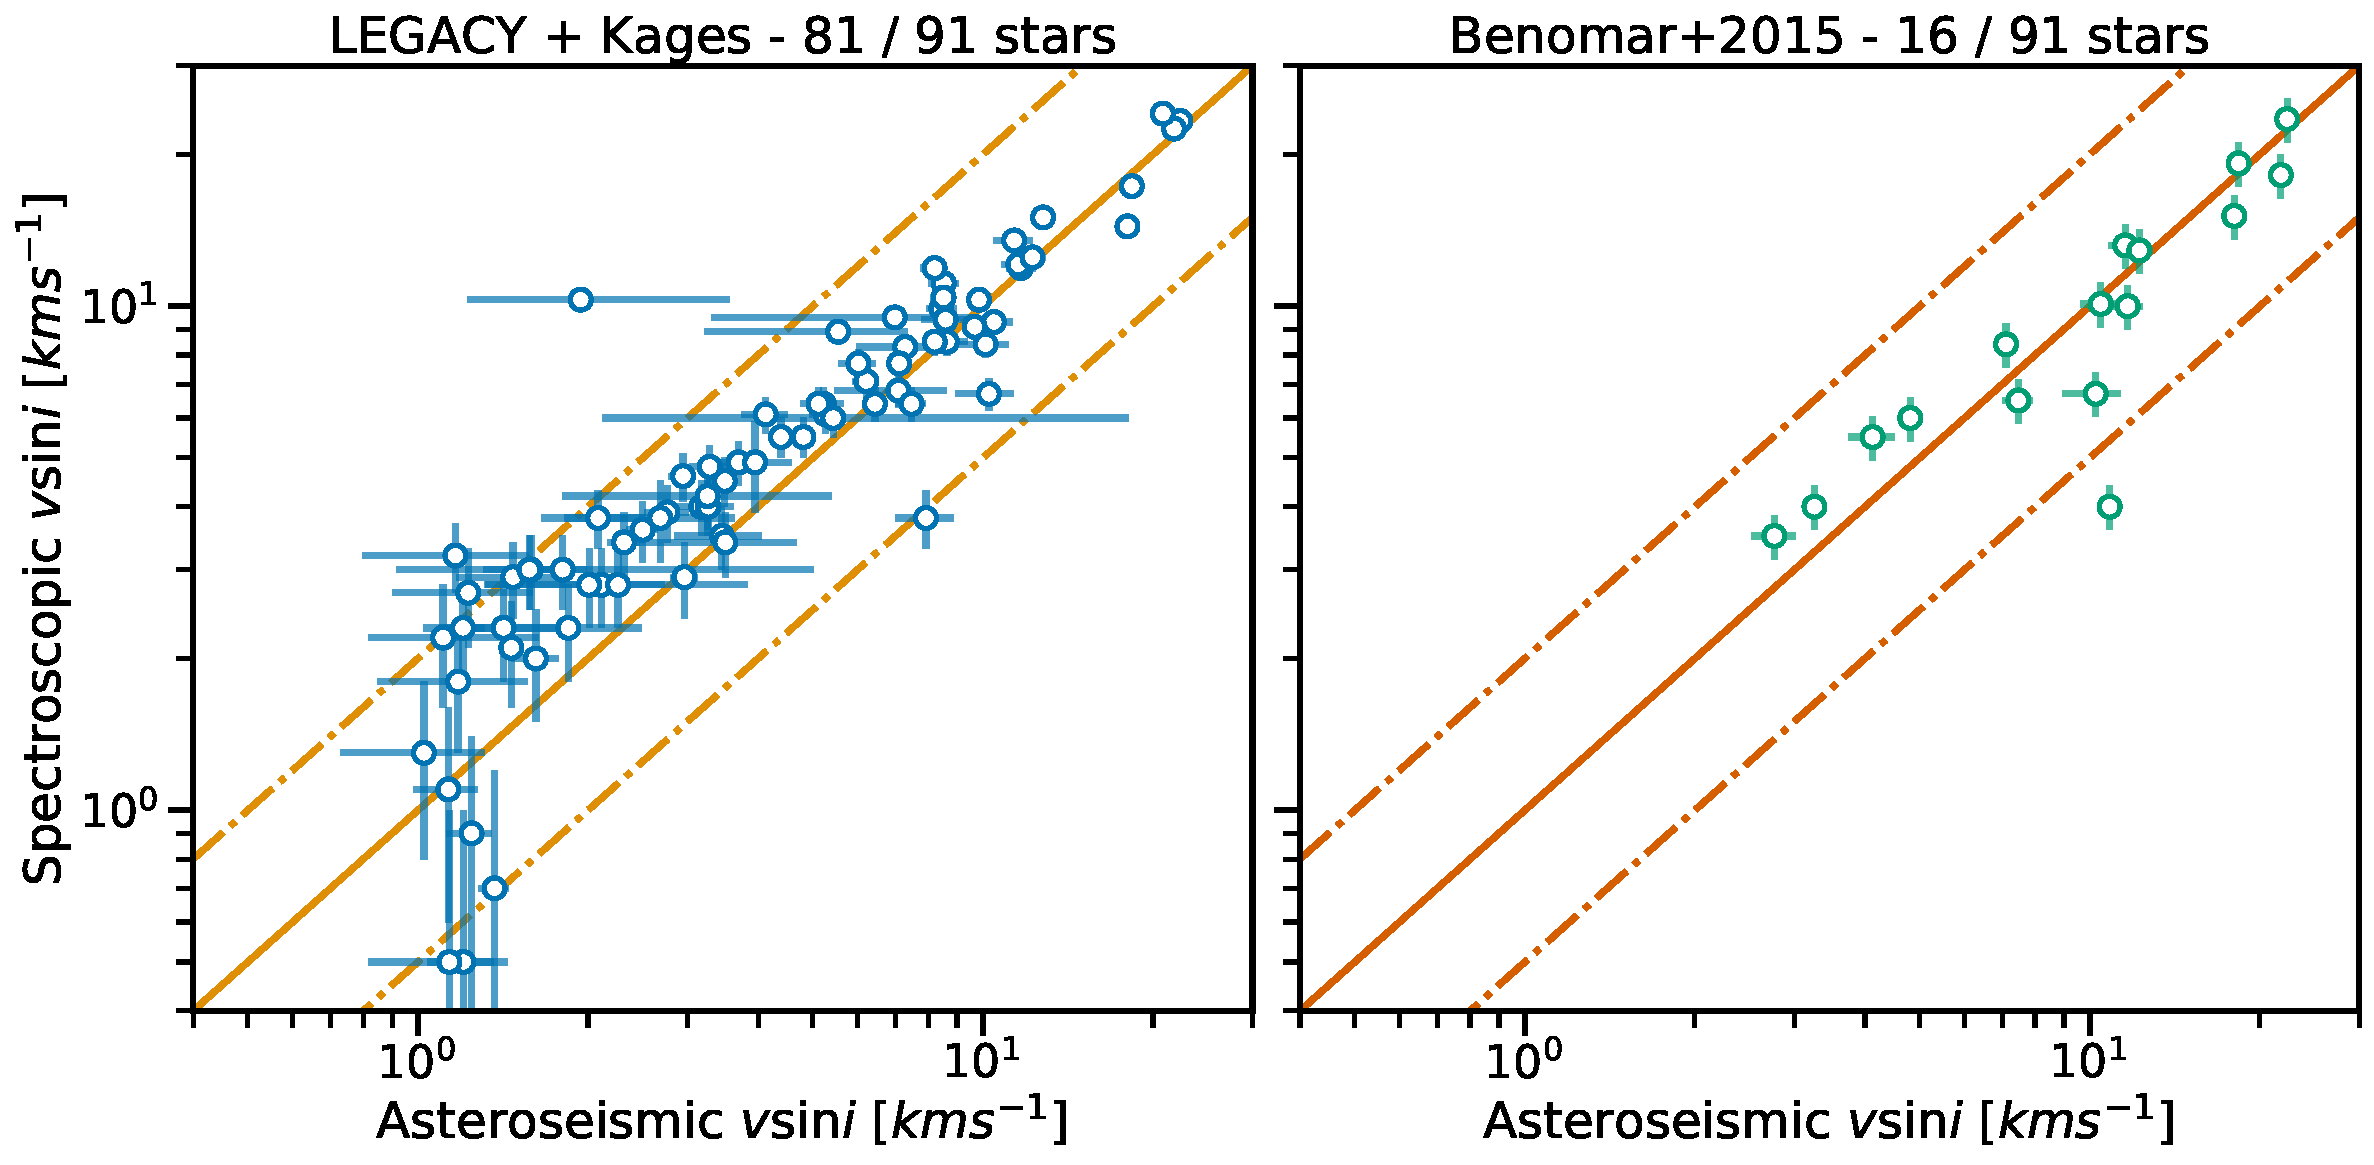
\includegraphics[width=\textwidth]{Images/vsini-comparison.pdf}
	\caption{Comparisons between asteroseismic and spectroscopic measures of projected surface rotation, $\textrm{v}\sin(i)$. All asteroseismic (x-axis) values are from this work, all spectroscopic (y-axis) values are from the literature. \textit{Left}: comparisons to 81 stars values reported in LEGACY and Kages. \textit{Right}: comparisons to 16 stars observed by \cite{benomar+2015}. Asteroseismic values are transformed from projected splitting ($\nu_s\sin(i)$) using the asteroseismic radius measurements presented in LEGACY and Kages. The solid lines indicate the 1:1 line, while the dash-dotted lines represent the 2:1 and 1:2 lines.}
	\label{fig:vsinilit}
\end{figure*}

We also repeated the \cite{nielsen+2015} comparison of asteroseismic rotation rates to surface rotation rates, using surface rotation measurements from \cite{nielsen+2013} and \cite{garcia+2014}. Figure \ref{fig:protlit} shows comparisons for 48 stars with rotation rates from both techniques, including 4 from the original \cite{nielsen+2015} sample. Rotation from spot-modulation are subject to measuring multiples of the true rotation rate, unlike an asteroseismic analysis \cite{mcquillan+2014}, and therefore some stars may appear at the 2:1 and 1:2 lines on the Figure.

We repeated the analysis in \cite{nielsen+2015} by fitting a line of the form $P_{\rm surf} = m \times P_{\rm seis}$. For the purposes of this fit we used the larger of the asymmetrical uncertainties on the seismic rotation from this work. In order to avoid biasing the fit due to outliers, we only included stars below the 1.8:1 line.

Our fit found a value of $m = 0.96\pm0.03$, showing a close agreement ($< 2\sigma$) between asteroseismic and surface rotation rates on a population level. Of the 40 stars that were part of this analysis, 21 had a median value of $P_{\rm s} < 0.5$ in the gyrochronology analysis. We repeated the model fit for these stars only, and found a value of $m = 0.96 \pm 0.04$. As we find no statistically significant deviation, we conclude that our asteroseismic ensemble is in agreement with surface rotation measurements of these stars, and can therefore be used to draw inferences about gyrochronology.

The overall agreement within the ensemble between the photometric measures of surface rotation and the asteroseismic rotation rates is in line with previous studies of Sun-like stars \cite{gizon+2013, chaplin+2013, nielsen+2015, benomar+2015}, where different measures of rotation appear indistinguishable.
Individual deviations from this agreement, as appears to be the case for a number of stars that lie distinctly off the bisector, may warrant a more in-depth analysis, which we leave to future work.

\subsection{Asteroseismic detection biases}

\section{Verifying consequences for gyrochronology}
\subsection{Rotational models for different stellar types}
Of the 73 stars for which posterior probability distributions of $P_{\rm s}$ were obtained, 4 were potential sub-giants, 22 were `hot' stars, and 47 were main sequence stars. Different stellar types should hold different amounts of diagnostic information about the standard or WMB models. Our `hot' stars should hold little to no information, as they lie above the Kraft break, where traditional gyrochronology relations used to build the stellar models break down (specifically, they do not lose angular momentum with time). Similarly, the rotational evolution of sub-giant stars is dominated by envelope expansion, complicating the interpretation of rotation. 

Figure \ref{fig:modelresults} shows joint posterior distributions for $P_{\rm s}$ for the three different stellar types, as well as their cumulative distributions. Both the  4 sub-giant stars and the 22 `hot' stars marginally prefer the standard model. The 47 MS stars on the other hand were most strongly in favour of weakened magnetic braking and dominate the full joint posterior. When only considering these stars, $99.2\%$ of the joint probability fell below $P_{\rm{s}} = 0.5$, compared to $98.4\%$ for all 73 stars.

\subsection{Limits of our stellar models}\label{ssec:limits}
The models presented in \cite{vansaders+2019} are constructed for metallicities of $-0.4 < \rm{[Fe/H]} < 0.4\, \rm{dex}$, in steps of $0.1\, \rm {dex}$. Our sample of 91 stars contained 4 stars with metallicities below $-0.4\, \rm{dex}$, which are shown as shaded symbols in Figure \ref{fig:fullmodels}. Of these 4, 3 were included in our final sample of 73 stars used to evaluate our stellar models: KICs 7970740, 8684723 and KIC 9965715. All three are classed as MS stars, with metallicities of $-0.54 \pm 0.10$, $-0.42 \pm 0.10$ and $-0.44 \pm 0.18\, \rm {dex}$ respectively, placing them within $3\sigma$ of the metallicity limits of our stellar models. KICs 8684723 and 9965715 strongly agree with the WMB model, whereas KIC 7970740 weakly prefers the standard model. Excluding these stars was not found to significantly alter the joint posterior distribution shown in Figure \ref{fig:modelresults}.

Recently, \cite{amard+matt2020} compared different rotational evolution models \cite[][of which we use the former in this work]{vansaders+pinsonneault2013,matt+2015} while studying the effect metallicity has on rotation. They found that metal-rich stars spin down significantly more effectively than metal poor stars. The population of 73 stars used in our stellar model comparisons is roughly centered on a $\rm{[Fe/H]}$ of 0 $\rm dex$, with a spread of $~0.16\, \rm dex$, with no stars significantly above or below $\pm 0.4\, \rm dex$ (as discussed above). While differences in stellar rotational evolution as a function of metallicity in this region are still somewhat pronounced, they are much less so than for more metal-rich or poor stars \cite[see Figure 2][]{amard+matt2020}. However, for stars with $\feh < 0$, the \cite{matt+2015} model prescription sees stars spin down more slowly than the models used in this work (i.e. they will rotate faster at later ages). This work only explores the presence of weakened magnetic braking for a single braking law, and a comparison to the \cite{matt+2015} braking model will be explored in a future paper.

When constructing KDEs from our stellar model samples (see Section \ref{s:gyro}), we selected fixed resolutions (or band-widths) for the KDEs. In mass, the band-width of $0.02\, M_\odot$, was larger than the uncertainties of 24 of 73 stars used to construct our joint posterior. For the stars with the smallest uncertainties, this significantly limits the size of the KDE being evaluated (as subsections of the full stellar models are used to evaluate individual stars, for computational efficiency). In order to confirm that these stars do not significantly affect the ensemble's preference towards the WMB model, we recalculated the joint posterior distribution for $P_{\rm s}$, excluding stars with an uncertainty on mass smaller than the KDE band-width. While the 24 stars with small uncertainties do favour the WMB model, they do so very weakly, whereas the remaining 49 stars with larger uncertainties strongly favour the WMB model. Their removal from the total joint posterior probability does not significantly alter it from the distribution shown in Figure \ref{fig:modelresults}.

\subsection{Systematic uncertainties from asteroseismology}
In our model analysis, we used asteroseismic mass and age obtained using \texttt{BASTA}, as reported in LEGACY and Kages. Asteroseismic properties obtained through stellar models can be subject to systematic errors arising from differences in input physics and choice of stellar models not included in the reported statistical uncertainties. A quantification of these different systematic effects can be found in Section 4 of \cite{silvaaguirre+2015}, based on the Kages catalogue. Combining their reported median systematic uncertainties due to input physics results in median uncertainties of $20\%$ (up from $14\%)$ on age and $5\%$ (up from $3\%$) on mass for the Kages sample. For LEGACY, the median uncertainties are $18\%$ (up from $10\%)$ and $5.6\%$ (up from $4\%$) for age and mass respectively.

In order to check the effect of systematic seismic uncertainties on our results for gyrochronology, we re-ran our model analysis described in Section \ref{s:gyro} after inflating uncertainties on mass and age. We increased uncertainties by the fractional difference between the \texttt{BASTA} statistical uncertainties and the median full statistical and systematic uncertainties described above. For example, a LEGACY star with a mass of $2.0 \pm 0.5\, M_\odot$ would have its uncertainty inflated by $1.6\%$ of its mass, to $0.53\, M_\odot$.

The results we found by repeating our model analysis with inflated uncertainties on asteroseismic mass and age closely replicated those found in our initial analysis. Specifically: subgiants preferred the standard model, and MS stars strongly favoured the WMB model. The `hot' stars in this case slightly preferred the WMB model compared to the unaltered ensemble. The full joint posterior distribution for 73 stars still strongly favours of the WMB model even with the inflated uncertainties, including when considering only stars on the main sequence, when excluding stars outside the models' metallicity range, and when excluding stars with low uncertainties on mass (see Section \ref{ssec:limits}).

To further test the limits of this analysis, we reran our mixture model fit, this time only shifting the asteroseismic ages younger by the systematic uncertainty, and retaining the statistical uncertainty (i.e. the ages of LEGACY and Kages stars were reduced by $8\%$ and $6\%$ respectively). In this scenario where all asteroseismic ages are overestimated, `true' fast rotators at young ages would have been mistaken for fast rotators at old ages, suggesting the presence of weakened magnetic braking where none existed. Despite the shift in age, the results from this mixture model fit closely matched those found for the unaltered ensemble, finding $95.8\%$ of the total posterior probability to lie below $P_{\rm s} = 0.5$ (as opposed to $98.4\%$ for the unaltered ensemble). While the preference for the WMB model is slightly reduced, we conclude that the use of asteroseismic age is valid for the gyrochronology analyses presented in this work.

\subsection{Binaries and Planet Hosts}
For stars to be good probes of existing gyrochronology relations, their rotational evolution must occur in isolation. If a star interacts with a close binary companion (through tides, or a merger) the natural angular momentum loss can be disturbed, causing gyrochronology to mispredict ages \cite{leiner+2019, fleming+2019}. Between LEGACY and Kages, we have 8 known binaries. 

First, KIC 8379927, KIC 7510397, KIC 10454113 and KIC 9025370 are spectroscopic binaries. This does not affect the asteroseismic analysis, but may affect their rotational evolution. Of these, KICs 8379927, 7510397 and 9025370 were included in the gyrochronology analysis. None of them preferred one model strongly over the other, with all three finding flat posteriors for $P_{\rm s}$.
% This implies that they are not yet at the Rossby number where weakened magnetic braking is proposed to take place in the models used in this work.

Second, the binary pairs of KIC 9139151 \& 9139163 and 16 Cyg A \& B are individually observed binary components with wide orbital separations, so we do not expect their binarity to have affected their rotational evolution. 

While we chose not to account for star-planet tidal interactions in this work, we note that this may also disturb the natural stellar rotational evolution when tidal forces are at play \cite{maxted+2015,gallet+delorme2019, benbakoura+2019}, although this has been disputed by observations of asteroseismic planet hosts \cite{ceillier+2016}.\\

\subsection{Evidence for Weakened Magnetic Braking in the literature}
Weakened magnetic braking was first proposed by \cite{vansaders+2016}, in response to stars with spot rotation rates faster than expected from gyrochronology at their asteroseismic ages. This discrepancy was also indicated at around the same time in other studies of asteroseismic ages of main sequence stars \cite{nielsen+2015, angus+2015, davies+2015}. The theory of weakened magnetic braking has been both reinforced by recent studies \cite{metcalfe+egeland2019}, as well as disputed \cite{lorenzo-oliveira+2019}, at least at the critical Rossby number originally proposed.

As a sanity check that the evidence in favour of weakened magnetic braking presented in this work is independently robust, we recreated the joint posterior probability for $P_{\rm s}$, this time looking only at MS stars, and excluding any of the 22 stars that were included in the original \cite{vansaders+2016} sample. Of the 47 MS stars used to distinguish between stellar models, 16 were included in the \cite{vansaders+2016} sample. Both the 16 \cite{vansaders+2016} stars as well as the remaining MS stars favoured the WMB model, although the \cite{vansaders+2016} stars did so more strongly, not including any stars that favoured the standard model. Specifically, when considering only the \cite{vansaders+2016} stars, $96.3\%$ of the total joint probability lay below $P_{\rm s} = 0.5$, compared to $91.7\%$ when considering only those stars \emph{not} included in the \cite{vansaders+2016} study. The stars initially used to propose the WMB model are still those most strongly in favour of it even when using asteroseismic rotation rates only. 
% It is encouraging that the inclusion of older, more quiescent stars and the use of asteroseismic rotation rates finds the same conclusion.}

Finally, we comment on the results found by \cite{lorenzo-oliveira+2019}. Using spectroscopic rotation measurements of 14 solar twins, compared to grids of stellar models, they found marginal evidence favouring a standard rotational evolution. If weakened magnetic braking were to take place, it would most likely be outside the range of their sample, at $Ro_{\rm {crit}} \geq 2.29$, compared to the value of $1.97$ used in this work. Our sample does not overlap with theirs, so we can not directly compare to their results. However, our work does find statistical agreement between our asteroseismic rotation rates and ages, and a model of weakened magnetic braking at a critical Rossby number of $1.97$. While a comparison to models of different Rossby numbers is outside the scope of this study, the LEGACY and Kages rotation sample may facilitate such studies in the future.
